\hypertarget{dcscMsgBufferInterface_8h}{
\section{dcsc\-Msg\-Buffer\-Interface.h File Reference}
\label{dcscMsgBufferInterface_8h}\index{dcscMsgBufferInterface.h@{dcscMsgBufferInterface.h}}
}
The Message Buffer Interface. This file implements the \hyperlink{group__dcsc__msg__buffer__access}{Message Buffer Encoding}. 

{\tt \#include $<$linux/types.h$>$}\par


Include dependency graph for dcsc\-Msg\-Buffer\-Interface.h:\begin{figure}[H]
\begin{center}
\leavevmode
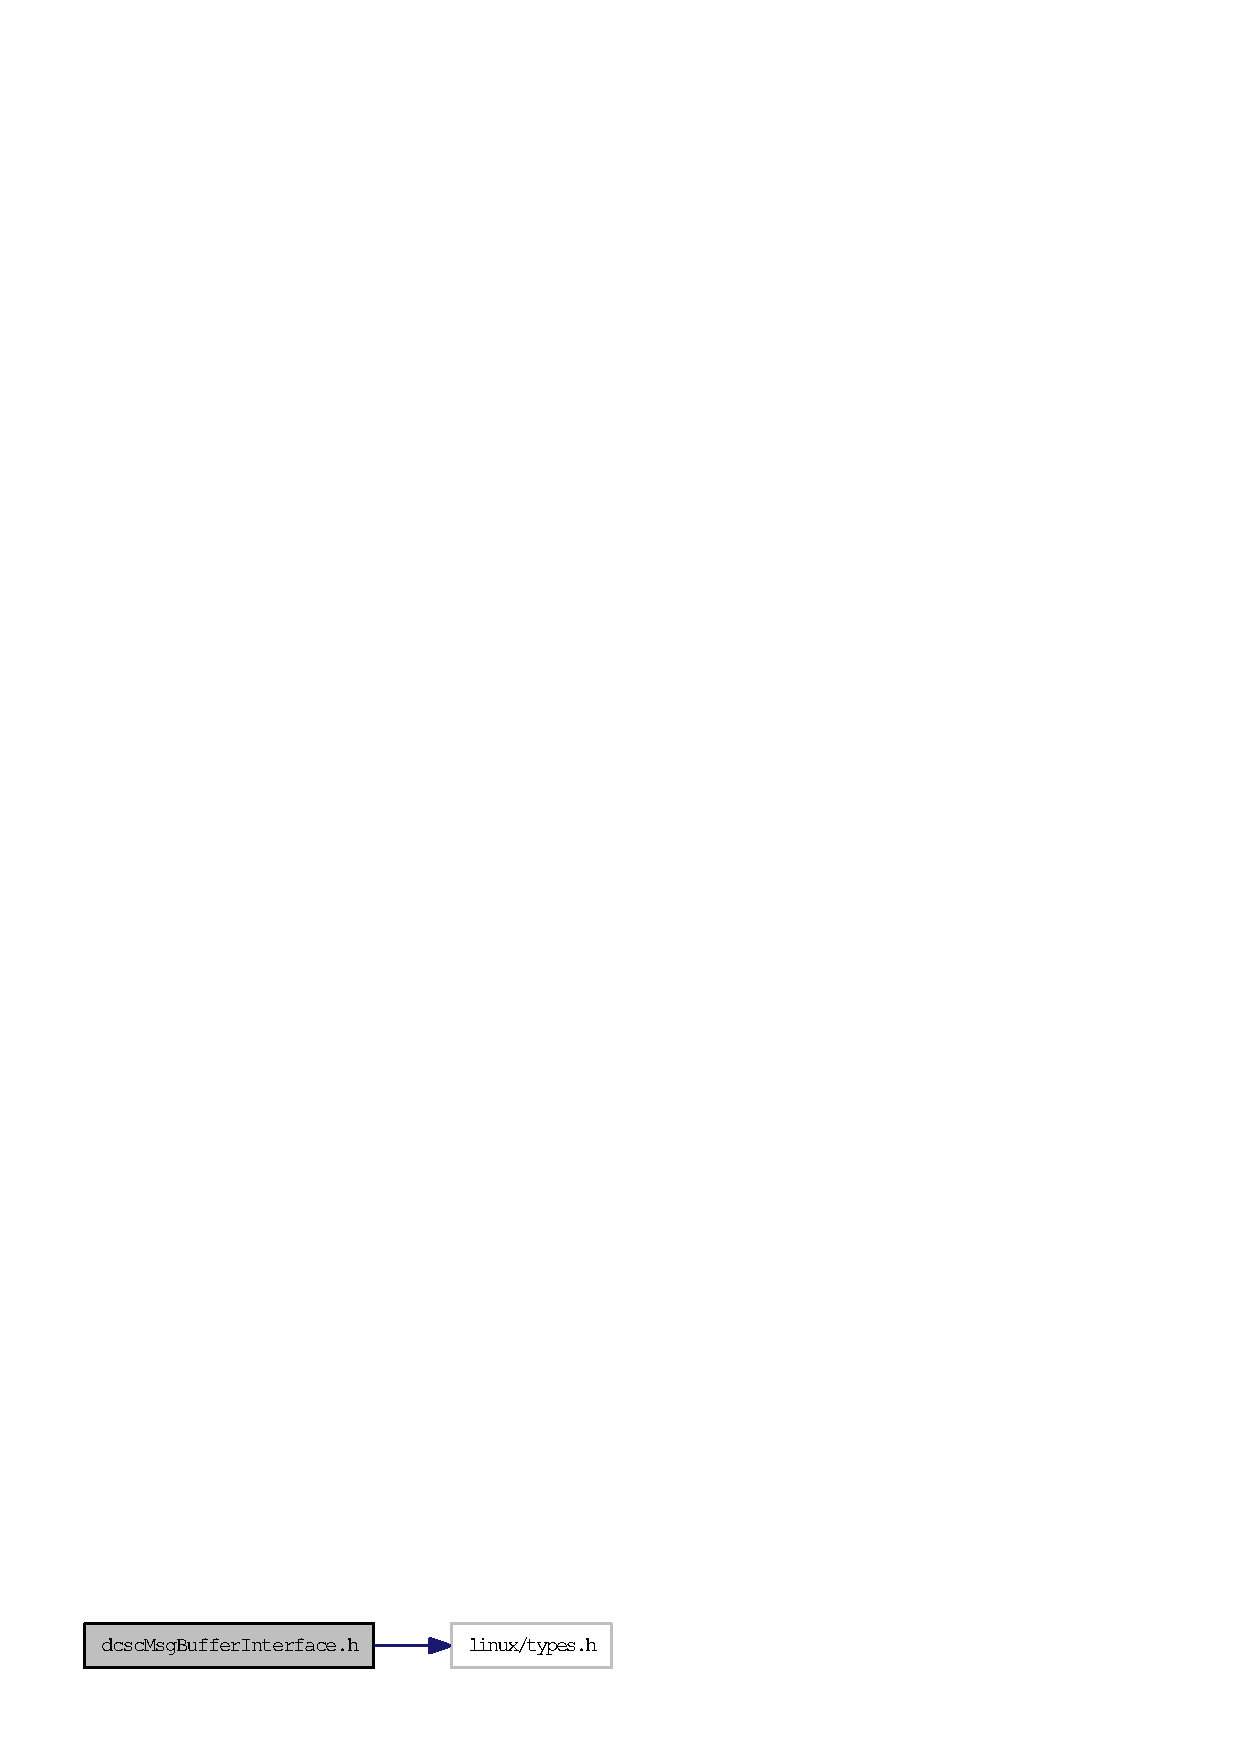
\includegraphics[width=149pt]{dcscMsgBufferInterface_8h__incl}
\end{center}
\end{figure}


This graph shows which files directly or indirectly include this file:\begin{figure}[H]
\begin{center}
\leavevmode
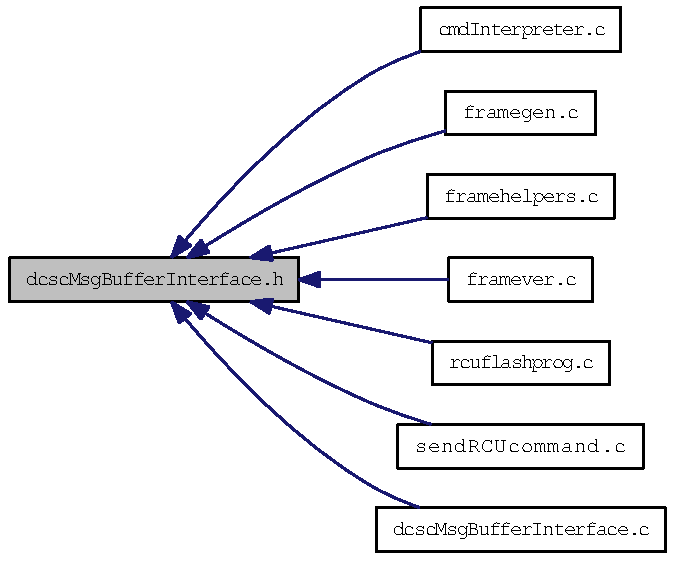
\includegraphics[width=180pt]{dcscMsgBufferInterface_8h__dep__incl}
\end{center}
\end{figure}
\subsection*{Data Structures}
\begin{CompactItemize}
\item 
struct \hyperlink{structdcscInitArguments__t}{dcsc\-Init\-Arguments\_\-t}
\begin{CompactList}\small\item\em Argument struct for extended initialization. \item\end{CompactList}\end{CompactItemize}
\subsection*{Format of the command sequence (32 bit words).}
The general format consists of a {\em header word\/}, the payload, a {\em block marker\/} and an {\em end marker\/}. The command can contain more than one block, each of them terminated by the {\em block marker\/}.

 Words 1 (information word) to n+2 (block marker) are considered to be programming blocks. A sequence of an arbitrary number of programming blocks is terminated by the end marker word. This is only limited by the size of the MIB. By now the dcsc\-Msg\-Buffer\-Interface interface uses only one programming block per sequence.

{\bf Header Word Version 2:} This is the current format\begin{itemize}
\item Bit 0-5 : command id\item Bit 6-15 : number of words(excluding the information and marker words)\item Bit 16-23: block number\item Bit 24-25: data format\item Bit 26 : flash mode if set\end{itemize}


The firmware has an inbuilt check for Bit 28-31, only 0x0 or 0x8 to 0xf are allowed for the 4 MSBs. Check the section 'Message Buffer Header Format Version' below.

{\bf Header Word Version 1:} this format is specified for backward compatibility only\begin{itemize}
\item Bit 0 - 15: number of words in the programming block including both information and marker word\item Bit 28- 31: command id\end{itemize}


{\bf Command IDs used by the interface:} \begin{CompactItemize}
\item 
\#define \hyperlink{dcscMsgBufferInterface_8h_6030c0d300916fd8ca54d740bbddd58a}{SINGLE\_\-READ}~0x1
\begin{CompactList}\small\item\em Code for the 'single read' command. \item\end{CompactList}\item 
\#define \hyperlink{dcscMsgBufferInterface_8h_155e21b5b6b1a7ee2ff293e43b2647af}{SINGLE\_\-WRITE}~0x2
\begin{CompactList}\small\item\em Code for the 'single write' command. \item\end{CompactList}\item 
\#define \hyperlink{dcscMsgBufferInterface_8h_a91382f3c0cd13e011f70c5f50d088f3}{MULTI\_\-READ}~0x3
\begin{CompactList}\small\item\em Code for the 'multiple read' command. \item\end{CompactList}\item 
\#define \hyperlink{dcscMsgBufferInterface_8h_dcd13dece10a23c37b7ac2a253781625}{MULTI\_\-WRITE}~0x4
\begin{CompactList}\small\item\em Code for the 'multiple write' command. \item\end{CompactList}\item 
\#define \hyperlink{dcscMsgBufferInterface_8h_71c4360ee488f413767765dd074cb92c}{RANDOM\_\-READ}~0x5
\begin{CompactList}\small\item\em Code for the 'random read' command. \item\end{CompactList}\item 
\#define \hyperlink{dcscMsgBufferInterface_8h_63a1fcd9162178ede0cbd908ed592038}{RANDOM\_\-WRITE}~0x6
\begin{CompactList}\small\item\em Code for the 'random write' command. \item\end{CompactList}\item 
\#define \hyperlink{dcscMsgBufferInterface_8h_75c771d18b83c211d2acccb56d2168be}{FLASH\_\-ERASEALL}~0x21
\begin{CompactList}\small\item\em Erase the flash completely. \item\end{CompactList}\item 
\#define \hyperlink{dcscMsgBufferInterface_8h_e30e07831b0e50dfd84e128a1317ba6a}{FLASH\_\-ERASE\_\-SEC}~0x22
\begin{CompactList}\small\item\em Erase one sector of the flash The command is specific to the rcu flash access, available since version 2.2. \item\end{CompactList}\item 
\#define \hyperlink{dcscMsgBufferInterface_8h_2dd7ad391d9119b630d0774285d720e8}{FLASH\_\-MULTI\_\-ERASE}~0x24
\begin{CompactList}\small\item\em Erase multiple sectors of the flash. \item\end{CompactList}\item 
\#define \hyperlink{dcscMsgBufferInterface_8h_9f8860f817da497ce396878c1dc143ea}{FLASH\_\-READID}~0x28
\begin{CompactList}\small\item\em Read the ID of the flash. \item\end{CompactList}\item 
\#define \hyperlink{dcscMsgBufferInterface_8h_9b890baacac98cc88ef06e9032a40e34}{FLASH\_\-RESET}~0x30
\begin{CompactList}\small\item\em Code for the flash reset command. \item\end{CompactList}\end{CompactItemize}
\subsection*{Message Buffer Header Format Version.}
Version handling has been introduced in firmware version 2.

\small\begin{alltt}
 Bit 28-31 of message buffer header
 0x0     : not used
 0x1-0x7 : version 1 (bit 31==0, other bits arbitrary)
 0xa     : version 2
 0xf     : Feeserver CE command
 \end{alltt}\normalsize 


{\bf Some helper defines} for the version decoding: \begin{CompactItemize}
\item 
\#define \hyperlink{group__dcsc__msg__buffer__access_gd47e658eba41557f654f0f9284c97317}{MSGBUF\_\-VERSION\_\-1\_\-MASK}~0x70000000
\begin{CompactList}\small\item\em Mask to extract Message Buffer Version 1 command ids. \item\end{CompactList}\item 
\#define \hyperlink{group__dcsc__msg__buffer__access_g4fc7f5db2448d65028809260a6d7879f}{MSGBUF\_\-VERSION\_\-2}~0xa0000000
\begin{CompactList}\small\item\em Message Buffer Version 2.0 id. \item\end{CompactList}\item 
\#define \hyperlink{group__dcsc__msg__buffer__access_gbe9b5c0065d5ca89ab3c3af7723c5340}{MSGBUF\_\-VERSION\_\-2\_\-2}~0xb0000000
\begin{CompactList}\small\item\em Message Buffer Version 2.2 id. \item\end{CompactList}\item 
\#define \hyperlink{group__dcsc__msg__buffer__access_g4922cdfb6125eef890c22cadeb1a4522}{FEESERVER\_\-CMD}~0xf0000000
\begin{CompactList}\small\item\em Fee\-Server command id. \item\end{CompactList}\end{CompactItemize}
\subsection*{Format of the command result (32 bit words).}
The result given in the MRB has the format:

\small\begin{alltt}
 ============================================
 1.information word (same format as above)
 2.status word
 3.- n: the data words follow
 Bit 0-15 of the information word contain the number of words in the buffer
          including status and information word. There is no end marker\end{alltt}\normalsize 


\small\begin{alltt} Status word: = 0 if no error
 Bit 15: set if any error
 \end{alltt}\normalsize 
 The interface uses the following defines to interprete the error bits: \begin{CompactItemize}
\item 
\#define \hyperlink{group__dcsc__msg__buffer__access_g08c36f682621c241c61818a20deb25c1}{MSGBUF\_\-STATUS\_\-NOMARKER}~0x01
\begin{CompactList}\small\item\em Status Word Bit 0: missing marker. \item\end{CompactList}\item 
\#define \hyperlink{group__dcsc__msg__buffer__access_gc30e76b52c140c354f56d34019c7f1d2}{MSGBUF\_\-STATUS\_\-NOENDMRK}~0x02
\begin{CompactList}\small\item\em Status Word Bit 1: missing end marker. \item\end{CompactList}\item 
\#define \hyperlink{group__dcsc__msg__buffer__access_g4eee888217162b8a35eb12d67cb4693b}{MSGBUF\_\-STATUS\_\-NOTGTASW}~0x04
\begin{CompactList}\small\item\em Status Word Bit 2: no target answer (something wrong with the RCU or not connected). \item\end{CompactList}\item 
\#define \hyperlink{group__dcsc__msg__buffer__access_g2c69c8f183428cc8448002ccbb40223f}{MSGBUF\_\-STATUS\_\-NOBUSGRT}~0x08
\begin{CompactList}\small\item\em Status Word Bit 3: no bus grant (no access to the bus on dcs board). \item\end{CompactList}\item 
\#define \hyperlink{group__dcsc__msg__buffer__access_g63adfcc12380aecaee776059a90bae31}{MSGBUF\_\-STATUS\_\-OLDFORMAT}~0X10
\begin{CompactList}\small\item\em Status Word Bit 5: old message buffer format (prior to v2 with rcu-sh version v1.0). \item\end{CompactList}\end{CompactItemize}
\subsection*{API methods: Initialization and general methods.}
\begin{CompactItemize}
\item 
\#define \hyperlink{group__dcsc__msg__buffer__access_gce40b0def5fb1f60ecebe3d5c07dceb5}{DCSC\_\-INIT\_\-FORCE\_\-V1}~0x0001
\begin{CompactList}\small\item\em Initialization flag: force message buffer format version v1 This sets the encoding to version 1 fixed rather than trying to get the correct firmware version. \item\end{CompactList}\item 
\#define \hyperlink{group__dcsc__msg__buffer__access_g24923a207203a43bfd322e7116edf028}{DCSC\_\-INIT\_\-FORCE\_\-V2}~0x0002
\begin{CompactList}\small\item\em Initialization flag: force message buffer format version v2. \item\end{CompactList}\item 
\#define \hyperlink{group__dcsc__msg__buffer__access_g1283f28b3ca2f03f4cfef9a0f8a8ce40}{DCSC\_\-INIT\_\-ENCODE}~0x0100
\begin{CompactList}\small\item\em Initialization flag: write block to device/file but do not execute. \item\end{CompactList}\item 
\#define \hyperlink{group__dcsc__msg__buffer__access_g1bf79fbd2d8c4bcfbed37007a5e9d4b0}{DCSC\_\-INIT\_\-APPEND}~0x0200
\begin{CompactList}\small\item\em Initialization flag: Append to file. \item\end{CompactList}\item 
\#define \hyperlink{group__dcsc__msg__buffer__access_g3a969c22c4b8fc27c201023112f70bb7}{DCSC\_\-SUPPR\_\-STDERR}~0x0400
\begin{CompactList}\small\item\em Initialization flag: suppress stderr output. \item\end{CompactList}\item 
\#define \hyperlink{group__dcsc__msg__buffer__access_g1d0799f8bf0c0b77db6155e5d78a4619}{DCSC\_\-SKIP\_\-DRV\_\-ADPT}~0x1000
\begin{CompactList}\small\item\em Initialization flag: skip automatic adaption to driver properties. \item\end{CompactList}\item 
typedef \hyperlink{structdcscInitArguments__t}{dcsc\-Init\-Arguments\_\-t} \hyperlink{group__dcsc__msg__buffer__access_gc35123ecbeaf4345c7ea161d1d31b500}{Tdcsc\-Init\-Arguments}
\begin{CompactList}\small\item\em Type definition for extended initialization parameters. \item\end{CompactList}\item 
int \hyperlink{group__dcsc__msg__buffer__access_gfc4448a8f5f9654cf54ad494f1558594}{init\-Rcu\-Access} (const char $\ast$p\-Device\-Name)
\begin{CompactList}\small\item\em Initialize the interface. \item\end{CompactList}\item 
int \hyperlink{group__dcsc__msg__buffer__access_g95f13464dd4da9231a53e7adbb0e7d4e}{init\-Rcu\-Access\-Ext} (const char $\ast$p\-Device\-Name, \hyperlink{structdcscInitArguments__t}{Tdcsc\-Init\-Arguments} $\ast$p\-Arg)
\begin{CompactList}\small\item\em Extended initialization. \item\end{CompactList}\item 
int \hyperlink{group__dcsc__msg__buffer__access_gac62a9e57c67af4cb9178b4426ec12fb}{release\-Rcu\-Access} ()
\begin{CompactList}\small\item\em Close the device and release internal data structures. \item\end{CompactList}\item 
void \hyperlink{group__dcsc__msg__buffer__access_g919bc832f5a0e82c07cfafd699b1b2ea}{print\-Driver\-Info} (int i\-Verbosity)
\begin{CompactList}\small\item\em Get driver info from the driver and print it. \item\end{CompactList}\item 
void \hyperlink{group__dcsc__msg__buffer__access_g0adb3aacb8d7ad32ceabe66a9dcbb401}{start\-Simulation} ()
\begin{CompactList}\small\item\em Start register simulation. \item\end{CompactList}\item 
void \hyperlink{group__dcsc__msg__buffer__access_gd871881385919aff64a8b679984cd018}{stop\-Simulation} ()
\begin{CompactList}\small\item\em Stop the simulation. \item\end{CompactList}\item 
void \hyperlink{group__dcsc__msg__buffer__access_gb54d216419ff2c191363373bef5f9cfa}{reset\-Simulation} ()
\begin{CompactList}\small\item\em Reset the simulation. \item\end{CompactList}\end{CompactItemize}
\subsection*{Interface debug options}
The debug output of the interface can be adjusted by a couple of flags. Flags can be changed by the \hyperlink{group__dcsc__msg__buffer__access_g36bb01dae6dd6edf579fe9878f9c6a20}{set\-Debug\-Option\-Flag}, \hyperlink{group__dcsc__msg__buffer__access_g41201fc4dd5608bce4261b34eec28ca4}{clear\-Debug\-Option\-Flag} and \hyperlink{group__dcsc__msg__buffer__access_gc07186b103fbe4c39531665c95e22c7e}{set\-Debug\-Options} functions. \begin{CompactItemize}
\item 
\#define \hyperlink{group__dcsc__msg__buffer__access_gdcd41743796fdb5a280fc3914121eb05}{PRINT\_\-COMMAND\_\-BUFFER}~0x01
\begin{CompactList}\small\item\em Print the command buffer before writing to the MIB. \item\end{CompactList}\item 
\#define \hyperlink{group__dcsc__msg__buffer__access_gcbc0bfb0d39b96550d664a58aa705cbb}{PRINT\_\-RESULT\_\-BUFFER}~0x02
\begin{CompactList}\small\item\em Print the MRB after executing the command. \item\end{CompactList}\item 
\#define \hyperlink{group__dcsc__msg__buffer__access_g9eba95d21cfe8d57e7d52cadc13e1b91}{CHECK\_\-COMMAND\_\-BUFFER}~0x04
\begin{CompactList}\small\item\em Test the MIB after writing the command buffer to it. \item\end{CompactList}\item 
\#define \hyperlink{group__dcsc__msg__buffer__access_g4115ae88155913f9a07bfbbd995f5e4f}{IGNORE\_\-BUFFER\_\-CHECK}~0x08
\begin{CompactList}\small\item\em Ignore the result of the MIB read back and check. \item\end{CompactList}\item 
\#define \hyperlink{group__dcsc__msg__buffer__access_gc3ceb106888209dd1796a27d49f567d8}{PRINT\_\-REGISTER\_\-ACCESS}~0x10
\begin{CompactList}\small\item\em Print access to the control registers. \item\end{CompactList}\item 
\#define \hyperlink{group__dcsc__msg__buffer__access_g2f996fd7aaf5d3df34642fc4dcd9ef66}{PRINT\_\-COMMAND\_\-RESULT}~0x20
\begin{CompactList}\small\item\em Print the result of the command. \item\end{CompactList}\item 
\#define \hyperlink{group__dcsc__msg__buffer__access_g36c838823c9602c6a0f6efd1fe135b18}{PRINT\_\-SPLIT\_\-DEBUG}~0x40
\begin{CompactList}\small\item\em Print split info for multiple operations. \item\end{CompactList}\item 
\#define \hyperlink{group__dcsc__msg__buffer__access_g6fe994d64da543fe875682bb79b5d585}{DBG\_\-FILE\_\-CONVERT}~0x80
\begin{CompactList}\small\item\em Print debug information on the file conversion. \item\end{CompactList}\item 
\#define \hyperlink{group__dcsc__msg__buffer__access_g5d966eba98a480141a4145615ca3ea15}{PRINT\_\-RESULT\_\-HUMAN\_\-READABLE}~0x100
\begin{CompactList}\small\item\em Print the status bits human readable. \item\end{CompactList}\item 
\#define \hyperlink{group__dcsc__msg__buffer__access_g7eaf88fd984d7f7c8c760dce4cb355d1}{DBG\_\-CHECK\_\-COMMAND}~0x400
\begin{CompactList}\small\item\em Print debug information concerning the wait ('check') command. \item\end{CompactList}\item 
\#define \hyperlink{group__dcsc__msg__buffer__access_gf34c3c30400c83a97dd0deadaead479c}{DBG\_\-DEFAULT}~PRINT\_\-RESULT\_\-HUMAN\_\-READABLE
\begin{CompactList}\small\item\em The default debug flags. \item\end{CompactList}\end{CompactItemize}
\subsection*{Interface error codes.}
The interface uses in general the error codes in errno.h. In addition to that a few more are defined which reflect the error returned in the MRB status word. \begin{CompactItemize}
\item 
\#define \hyperlink{group__dcsc__msg__buffer__access_g2a64137d0941a60d8a7c65c60cf270d1}{EMISS\_\-MARKER}~0x1001
\begin{CompactList}\small\item\em Error indicates a missing marker in the message buffer command. \item\end{CompactList}\item 
\#define \hyperlink{group__dcsc__msg__buffer__access_g0003c432c9b704625105bb7fda5e875e}{EMISS\_\-ENDMARKER}~0x1002
\begin{CompactList}\small\item\em Error indicates a missing end marker at the and of the message buffer command block. \item\end{CompactList}\item 
\#define \hyperlink{group__dcsc__msg__buffer__access_g784f97ba20855df7fdcfb165ba30ba4c}{ENOTARGET}~0x1003
\begin{CompactList}\small\item\em Error in the communication between DCS board and RCU motherboard, no target answer. \item\end{CompactList}\item 
\#define \hyperlink{group__dcsc__msg__buffer__access_g6a6e1cfe5a616e5424852a4519bd47a9}{ENOBUSGRANT}~0x1004
\begin{CompactList}\small\item\em Error on the DCS board internally, no bus grant. \item\end{CompactList}\item 
\#define \hyperlink{group__dcsc__msg__buffer__access_g78f0a660b0b99a94de586d9174999492}{EOLDFORMAT}~0x1005
\begin{CompactList}\small\item\em Error indicates an old message buffer v1 format. \item\end{CompactList}\end{CompactItemize}
\subsection*{Read/write access}
\begin{CompactItemize}
\item 
enum \{ \par
\hyperlink{group__dcsc__msg__buffer__access_gg0411cd49bb5b71852cecd93bcbf0ca2d369f66006fcdc9be0ebe0e56d0dce6c9}{e\-Unknown\-Spec} =  0, 
\hyperlink{group__dcsc__msg__buffer__access_gg0411cd49bb5b71852cecd93bcbf0ca2d1d0f8ecdb452c7ff543d75a98c9cc6b4}{e\-Version}, 
\hyperlink{group__dcsc__msg__buffer__access_gg0411cd49bb5b71852cecd93bcbf0ca2d203d36b00bb0c66542bfbb41283bca1f}{e\-Command}, 
\hyperlink{group__dcsc__msg__buffer__access_gg0411cd49bb5b71852cecd93bcbf0ca2d5c578774a774b0e23c176c8a045b742b}{e\-Nof\-Words}, 
\par
\hyperlink{group__dcsc__msg__buffer__access_gg0411cd49bb5b71852cecd93bcbf0ca2d6678ba12b9d3d2b765aa92a0d12bc1b7}{e\-Packed}
 \}
\begin{CompactList}\small\item\em Operation specifier for the \hyperlink{group__dcsc__msg__buffer__access_g975e68b162a4d0786e1902c895349b02}{dcsc\-Get\-Header\-Attribute} function. \item\end{CompactList}\item 
int \hyperlink{group__dcsc__msg__buffer__access_g5b2ecab6b0a6383afebde1ea486dae43}{rcu\-Single\-Write} (\_\-\_\-u32 address, \_\-\_\-u32 data)
\begin{CompactList}\small\item\em Write a single location (32bit word). \item\end{CompactList}\item 
int \hyperlink{group__dcsc__msg__buffer__access_g339b5922513d0f0211d7962234faa24f}{rcu\-Single\-Read} (\_\-\_\-u32 address, \_\-\_\-u32 $\ast$p\-Data)
\begin{CompactList}\small\item\em Read a single location (32bit word). \item\end{CompactList}\item 
int \hyperlink{group__dcsc__msg__buffer__access_ge20afbfc92c897546e37126188804309}{rcu\-Multiple\-Write} (\_\-\_\-u32 address, \_\-\_\-u32 $\ast$p\-Data, int i\-Size, int i\-Data\-Size)
\begin{CompactList}\small\item\em Write a number of 32bit words beginning at a location. \item\end{CompactList}\item 
int \hyperlink{group__dcsc__msg__buffer__access_g602216accce6913989f8b04b36157cd6}{rcu\-Multiple\-Read} (\_\-\_\-u32 address, int i\-Size, \_\-\_\-u32 $\ast$p\-Data)
\begin{CompactList}\small\item\em Read a number of 32bit words beginning at a location. \item\end{CompactList}\item 
int \hyperlink{group__dcsc__msg__buffer__access_gf7be7371f7530e8eb6e07e6f0d969b04}{dcsc\-Provide\-Message\-Buffer} (\_\-\_\-u32 $\ast$$\ast$pp\-Buffer, int $\ast$p\-Size)
\begin{CompactList}\small\item\em Provide the message buffer for direct access. \item\end{CompactList}\item 
int \hyperlink{group__dcsc__msg__buffer__access_g4f25fcb80c8fad99d5d72f96e72bd941}{dcsc\-Prepare\-Message\-Buffer} (\_\-\_\-u32 $\ast$$\ast$pp\-Buffer, int $\ast$p\-Size, unsigned int cmd\-ID, unsigned int flags)
\begin{CompactList}\small\item\em Prepare the message buffer for a specific command. \item\end{CompactList}\item 
int \hyperlink{group__dcsc__msg__buffer__access_g96f1fe73877d927a698a396df555767e}{dcsc\-Execute\-Command} (\_\-\_\-u32 $\ast$\hyperlink{dcscMsgBufferInterface_8c_7fe69f55846ac3a138c130665f1f1e49}{p\-Buffer}, int i\-Size, \_\-\_\-u32 $\ast$$\ast$pp\-Target, int $\ast$pp\-Target\-Size, unsigned int operation)
\begin{CompactList}\small\item\em Execute the message buffer command. \item\end{CompactList}\item 
int \hyperlink{group__dcsc__msg__buffer__access_g975e68b162a4d0786e1902c895349b02}{dcsc\-Get\-Header\-Attribute} (\_\-\_\-u32 \hyperlink{virtex__io_8h_f662138894a99f1d07d07f482b7c2691}{header}, int i\-Specifier)
\begin{CompactList}\small\item\em Extract a part of the header word according to the specifier. \item\end{CompactList}\item 
int \hyperlink{group__dcsc__msg__buffer__access_g8dac87332689e82a586ef04eed99d083}{dcsc\-Check\-Msg\-Block} (\_\-\_\-u32 $\ast$\hyperlink{dcscMsgBufferInterface_8c_7fe69f55846ac3a138c130665f1f1e49}{p\-Buffer}, int i\-Size, int i\-Verbosity)
\begin{CompactList}\small\item\em Check a message block for correct format. \item\end{CompactList}\end{CompactItemize}
\subsection*{Driver control functions}
\begin{CompactItemize}
\item 
enum \{ \par
\hyperlink{group__dcsc__msg__buffer__access_ggbed82baf7f470b522273a3e37c24c600da3c950575dcbbc7ca50d76a111d217d}{e\-Unknown\-Driver\-Cmd} = 0, 
\hyperlink{group__dcsc__msg__buffer__access_ggbed82baf7f470b522273a3e37c24c600c0b7933997697a647dbfb83d828142f3}{e\-Lock}, 
\hyperlink{group__dcsc__msg__buffer__access_ggbed82baf7f470b522273a3e37c24c600fc021c4ba87bb9763ec7f4e07855d8f9}{e\-Unlock}, 
\hyperlink{group__dcsc__msg__buffer__access_ggbed82baf7f470b522273a3e37c24c6001391714f3c5c8e7738e9b0e871dc3cce}{e\-Seize}, 
\par
\hyperlink{group__dcsc__msg__buffer__access_ggbed82baf7f470b522273a3e37c24c6001349887513e044eb25dceda6bc2c9429}{e\-Release}, 
\hyperlink{group__dcsc__msg__buffer__access_ggbed82baf7f470b522273a3e37c24c600be8853084b74223aab7a0a0c8150eb5a}{e\-Deactivate\-Lock}, 
\hyperlink{group__dcsc__msg__buffer__access_ggbed82baf7f470b522273a3e37c24c60052e15b8bac21d0241661e3caf289e745}{e\-Activate\-Lock}
 \}
\begin{CompactList}\small\item\em Operation ids for the \hyperlink{group__dcsc__msg__buffer__access_gb01774a452cb68f631a87d2d77ac79a5}{dcsc\-Lock\-Ctrl} function. \item\end{CompactList}\item 
int \hyperlink{group__dcsc__msg__buffer__access_gb01774a452cb68f631a87d2d77ac79a5}{dcsc\-Lock\-Ctrl} (int cmd)
\begin{CompactList}\small\item\em Lock the driver. \item\end{CompactList}\item 
int \hyperlink{group__dcsc__msg__buffer__access_g8dc96e96fb45e86a27c98fbe8d816edf}{dcsc\-Driver\-Debug} (unsigned int flags)
\begin{CompactList}\small\item\em Set debug flags for the driver. \item\end{CompactList}\end{CompactItemize}
\subsection*{Bus control functions}
\begin{CompactItemize}
\item 
enum \{ \par
\hyperlink{group__dcsc__msg__buffer__access_ggb04a0655cd1e3bcac5e8f48c18df1a5701615e05df0af61e9fae12f1b21e677d}{e\-Unknown\-Bus\-Ctrl} = 0, 
\hyperlink{group__dcsc__msg__buffer__access_ggb04a0655cd1e3bcac5e8f48c18df1a577b8222808ce70929afddb10c7855f13a}{e\-Enable\-Selectmap}, 
\hyperlink{group__dcsc__msg__buffer__access_ggb04a0655cd1e3bcac5e8f48c18df1a57e4c19a8b3abecb07f7e1a686e9e31b35}{e\-Disable\-Selectmap}, 
\hyperlink{group__dcsc__msg__buffer__access_ggb04a0655cd1e3bcac5e8f48c18df1a573b9d25a6fa4e461b6eb1756217e2ccdd}{e\-Enable\-Flash}, 
\par
\hyperlink{group__dcsc__msg__buffer__access_ggb04a0655cd1e3bcac5e8f48c18df1a577c7ba96930a1249cc2049d4427fd9ac9}{e\-Disable\-Flash}, 
\hyperlink{group__dcsc__msg__buffer__access_ggb04a0655cd1e3bcac5e8f48c18df1a57d12ce67d46f81ac74100f3d9a8058f25}{e\-Enable\-Msg\-Buf}, 
\hyperlink{group__dcsc__msg__buffer__access_ggb04a0655cd1e3bcac5e8f48c18df1a5702c0aacdb67187c6b37d3a42cdf857cc}{e\-Reset\-Firmware}, 
\hyperlink{group__dcsc__msg__buffer__access_ggb04a0655cd1e3bcac5e8f48c18df1a57d3e958eb3b288db3f4942dd3a81c6087}{e\-Read\-Ctrl\-Reg}, 
\par
\hyperlink{group__dcsc__msg__buffer__access_ggb04a0655cd1e3bcac5e8f48c18df1a578e3fd457e9da4ecb682532b1f64ca2e2}{e\-Check\-Selectmap}, 
\hyperlink{group__dcsc__msg__buffer__access_ggb04a0655cd1e3bcac5e8f48c18df1a574581ed60d70cf970eac090dd985e68e1}{e\-Check\-Flash}, 
\hyperlink{group__dcsc__msg__buffer__access_ggb04a0655cd1e3bcac5e8f48c18df1a57b8a5bc377b3c7d019be52e0da9e57565}{e\-Check\-Msg\-Buf}, 
\hyperlink{group__dcsc__msg__buffer__access_ggb04a0655cd1e3bcac5e8f48c18df1a57fa0c1e1d2d3baba10b94f02c4b2c7f01}{e\-Reset\-Flash}, 
\par
\hyperlink{group__dcsc__msg__buffer__access_ggb04a0655cd1e3bcac5e8f48c18df1a57298817c93fab57042b42b0c23d3efdc4}{e\-Flash\-ID}, 
\hyperlink{group__dcsc__msg__buffer__access_ggb04a0655cd1e3bcac5e8f48c18df1a5756591b8d17f10234722790d952ed8781}{e\-Flash\-Ctrl\-DCS}, 
\hyperlink{group__dcsc__msg__buffer__access_ggb04a0655cd1e3bcac5e8f48c18df1a574a96ce967a91331568455c580e4a2ca1}{e\-Flash\-Ctrl\-Actel}, 
\hyperlink{group__dcsc__msg__buffer__access_ggb04a0655cd1e3bcac5e8f48c18df1a57ec59997e5b2ac539cc85158012221f82}{e\-Enable\-Compression}, 
\par
\hyperlink{group__dcsc__msg__buffer__access_ggb04a0655cd1e3bcac5e8f48c18df1a57a371d588d9e5eb297b5e8c39d62bfe1c}{e\-Disable\-Compression}
 \}
\begin{CompactList}\small\item\em Command ids to the \hyperlink{group__dcsc__msg__buffer__access_gf74b29f8ded2feb57974c95e4863eac8}{rcu\-Bus\-Control\-Cmd} function. \item\end{CompactList}\item 
int \hyperlink{group__dcsc__msg__buffer__access_gf74b29f8ded2feb57974c95e4863eac8}{rcu\-Bus\-Control\-Cmd} (int i\-Cmd)
\begin{CompactList}\small\item\em Switch bits in the control register (firmware comstat). \item\end{CompactList}\item 
int \hyperlink{group__dcsc__msg__buffer__access_g7a5b0d57fbd0a68206468a01b0a63520}{msg\-Buf\-Read\-Register} (int reg)
\begin{CompactList}\small\item\em Read the value of a register from the register buffer. \item\end{CompactList}\item 
int \hyperlink{group__dcsc__msg__buffer__access_g82e19c9d34c7ecebcba115d2a6393b6c}{msg\-Buf\-Write\-Register} (int reg, unsigned char value)
\begin{CompactList}\small\item\em Write an 8 bit value to a register of the register buffer. \item\end{CompactList}\end{CompactItemize}
\subsection*{Flash control functions}
\begin{CompactItemize}
\item 
int \hyperlink{group__dcsc__msg__buffer__access_g88debbd24075d2031add9459e4d90e2b}{rcu\-Flash\-Write} (\_\-\_\-u32 address, \_\-\_\-u32 $\ast$p\-Data, int i\-Size, int i\-Data\-Size)
\begin{CompactList}\small\item\em Write to the RCU flash. \item\end{CompactList}\item 
int \hyperlink{group__dcsc__msg__buffer__access_g24164f14711ead31a7e542711f0a08b3}{rcu\-Flash\-Read} (\_\-\_\-u32 address, int i\-Size, \_\-\_\-u32 $\ast$p\-Data)
\begin{CompactList}\small\item\em Read a number of 16bit words from the flash memory. \item\end{CompactList}\item 
int \hyperlink{group__dcsc__msg__buffer__access_g78e6fc883a098cf548e9d0ba618ecb16}{rcu\-Flash\-Erase} (int start\-Sec, int stop\-Sec)
\begin{CompactList}\small\item\em Erase sectors of the flash. \item\end{CompactList}\end{CompactItemize}
\subsection*{Debug Message Control}
\begin{CompactItemize}
\item 
int \hyperlink{group__dcsc__msg__buffer__access_gc07186b103fbe4c39531665c95e22c7e}{set\-Debug\-Options} (int options)
\begin{CompactList}\small\item\em Set the debug options. \item\end{CompactList}\item 
int \hyperlink{group__dcsc__msg__buffer__access_g36bb01dae6dd6edf579fe9878f9c6a20}{set\-Debug\-Option\-Flag} (int of)
\begin{CompactList}\small\item\em Set a debug option flag. \item\end{CompactList}\item 
int \hyperlink{group__dcsc__msg__buffer__access_g41201fc4dd5608bce4261b34eec28ca4}{clear\-Debug\-Option\-Flag} (int of)
\begin{CompactList}\small\item\em clear a debug option flag. \item\end{CompactList}\item 
void \hyperlink{group__dcsc__msg__buffer__access_g1b3027d209be85e9a8fbd14864c4b442}{print\-Buffer\-Hex} (unsigned char $\ast$\hyperlink{dcscMsgBufferInterface_8c_7fe69f55846ac3a138c130665f1f1e49}{p\-Buffer}, int i\-Buffer\-Size, int word\-Size, const char $\ast$p\-Message)
\begin{CompactList}\small\item\em Print content of a buffer hexadecimal. \item\end{CompactList}\item 
void \hyperlink{group__dcsc__msg__buffer__access_gc44ca908f157f8de95b81638e298e08e}{print\-Buffer\-Hex\-Formatted} (unsigned char $\ast$\hyperlink{dcscMsgBufferInterface_8c_7fe69f55846ac3a138c130665f1f1e49}{p\-Buffer}, int i\-Buffer\-Size, int i\-Word\-Size, int i\-Words\-Per\-Row, int i\-Start\-Address, const char $\ast$p\-Message)
\begin{CompactList}\small\item\em Print content of a buffer hexadecimal formated with the address. \item\end{CompactList}\end{CompactItemize}


\subsection{Detailed Description}
The Message Buffer Interface. This file implements the \hyperlink{group__dcsc__msg__buffer__access}{Message Buffer Encoding}. 

\begin{Desc}
\item[Author:]Matthias Richter \end{Desc}
\begin{Desc}
\item[Date:]\end{Desc}


Definition in file \hyperlink{dcscMsgBufferInterface_8h-source}{dcsc\-Msg\-Buffer\-Interface.h}.

\subsection{Define Documentation}
\hypertarget{dcscMsgBufferInterface_8h_e30e07831b0e50dfd84e128a1317ba6a}{
\index{dcscMsgBufferInterface.h@{dcsc\-Msg\-Buffer\-Interface.h}!FLASH_ERASE_SEC@{FLASH\_\-ERASE\_\-SEC}}
\index{FLASH_ERASE_SEC@{FLASH\_\-ERASE\_\-SEC}!dcscMsgBufferInterface.h@{dcsc\-Msg\-Buffer\-Interface.h}}
\subsubsection[FLASH\_\-ERASE\_\-SEC]{\setlength{\rightskip}{0pt plus 5cm}\#define FLASH\_\-ERASE\_\-SEC~0x22}}
\label{dcscMsgBufferInterface_8h_e30e07831b0e50dfd84e128a1317ba6a}


Erase one sector of the flash The command is specific to the rcu flash access, available since version 2.2. 

of the DCSboard firmware. payload:\par
 1 data word: sector address 

Definition at line 180 of file dcsc\-Msg\-Buffer\-Interface.h.

Referenced by rcu\-Flash\-Erase().\hypertarget{dcscMsgBufferInterface_8h_75c771d18b83c211d2acccb56d2168be}{
\index{dcscMsgBufferInterface.h@{dcsc\-Msg\-Buffer\-Interface.h}!FLASH_ERASEALL@{FLASH\_\-ERASEALL}}
\index{FLASH_ERASEALL@{FLASH\_\-ERASEALL}!dcscMsgBufferInterface.h@{dcsc\-Msg\-Buffer\-Interface.h}}
\subsubsection[FLASH\_\-ERASEALL]{\setlength{\rightskip}{0pt plus 5cm}\#define FLASH\_\-ERASEALL~0x21}}
\label{dcscMsgBufferInterface_8h_75c771d18b83c211d2acccb56d2168be}


Erase the flash completely. 

The command is specific to the rcu flash access, available since version 2.2. of the DCSboard firmware. payload:\par
 no data words 

Definition at line 171 of file dcsc\-Msg\-Buffer\-Interface.h.

Referenced by rcu\-Flash\-Erase().\hypertarget{dcscMsgBufferInterface_8h_2dd7ad391d9119b630d0774285d720e8}{
\index{dcscMsgBufferInterface.h@{dcsc\-Msg\-Buffer\-Interface.h}!FLASH_MULTI_ERASE@{FLASH\_\-MULTI\_\-ERASE}}
\index{FLASH_MULTI_ERASE@{FLASH\_\-MULTI\_\-ERASE}!dcscMsgBufferInterface.h@{dcsc\-Msg\-Buffer\-Interface.h}}
\subsubsection[FLASH\_\-MULTI\_\-ERASE]{\setlength{\rightskip}{0pt plus 5cm}\#define FLASH\_\-MULTI\_\-ERASE~0x24}}
\label{dcscMsgBufferInterface_8h_2dd7ad391d9119b630d0774285d720e8}


Erase multiple sectors of the flash. 

The command is specific to the rcu flash access, available since version 2.2. of the DCSboard firmware. payload:\par
 2 data words: sector address and count 

Definition at line 189 of file dcsc\-Msg\-Buffer\-Interface.h.

Referenced by rcu\-Flash\-Erase().\hypertarget{dcscMsgBufferInterface_8h_9f8860f817da497ce396878c1dc143ea}{
\index{dcscMsgBufferInterface.h@{dcsc\-Msg\-Buffer\-Interface.h}!FLASH_READID@{FLASH\_\-READID}}
\index{FLASH_READID@{FLASH\_\-READID}!dcscMsgBufferInterface.h@{dcsc\-Msg\-Buffer\-Interface.h}}
\subsubsection[FLASH\_\-READID]{\setlength{\rightskip}{0pt plus 5cm}\#define FLASH\_\-READID~0x28}}
\label{dcscMsgBufferInterface_8h_9f8860f817da497ce396878c1dc143ea}


Read the ID of the flash. 

The command is specific to the rcu flash access, available since version 2.2. of the DCSboard firmware. payload:\par
 1 data word: 0 manufacturer id, 1 device id 

Definition at line 198 of file dcsc\-Msg\-Buffer\-Interface.h.

Referenced by rcu\-Flash\-ID().\hypertarget{dcscMsgBufferInterface_8h_9b890baacac98cc88ef06e9032a40e34}{
\index{dcscMsgBufferInterface.h@{dcsc\-Msg\-Buffer\-Interface.h}!FLASH_RESET@{FLASH\_\-RESET}}
\index{FLASH_RESET@{FLASH\_\-RESET}!dcscMsgBufferInterface.h@{dcsc\-Msg\-Buffer\-Interface.h}}
\subsubsection[FLASH\_\-RESET]{\setlength{\rightskip}{0pt plus 5cm}\#define FLASH\_\-RESET~0x30}}
\label{dcscMsgBufferInterface_8h_9b890baacac98cc88ef06e9032a40e34}


Code for the flash reset command. 

The command is specific to the rcu flash access, available since version 2.2. of the DCSboard firmware. payload:\par
 no data words 

Definition at line 207 of file dcsc\-Msg\-Buffer\-Interface.h.

Referenced by rcu\-Flash\-Reset().\hypertarget{dcscMsgBufferInterface_8h_a91382f3c0cd13e011f70c5f50d088f3}{
\index{dcscMsgBufferInterface.h@{dcsc\-Msg\-Buffer\-Interface.h}!MULTI_READ@{MULTI\_\-READ}}
\index{MULTI_READ@{MULTI\_\-READ}!dcscMsgBufferInterface.h@{dcsc\-Msg\-Buffer\-Interface.h}}
\subsubsection[MULTI\_\-READ]{\setlength{\rightskip}{0pt plus 5cm}\#define MULTI\_\-READ~0x3}}
\label{dcscMsgBufferInterface_8h_a91382f3c0cd13e011f70c5f50d088f3}


Code for the 'multiple read' command. 

payload:\par
\begin{itemize}
\item 32 bit address word\item 32 bit number of words \end{itemize}


Definition at line 141 of file dcsc\-Msg\-Buffer\-Interface.h.

Referenced by rcu\-Multiple\-Read\-Ext().\hypertarget{dcscMsgBufferInterface_8h_dcd13dece10a23c37b7ac2a253781625}{
\index{dcscMsgBufferInterface.h@{dcsc\-Msg\-Buffer\-Interface.h}!MULTI_WRITE@{MULTI\_\-WRITE}}
\index{MULTI_WRITE@{MULTI\_\-WRITE}!dcscMsgBufferInterface.h@{dcsc\-Msg\-Buffer\-Interface.h}}
\subsubsection[MULTI\_\-WRITE]{\setlength{\rightskip}{0pt plus 5cm}\#define MULTI\_\-WRITE~0x4}}
\label{dcscMsgBufferInterface_8h_dcd13dece10a23c37b7ac2a253781625}


Code for the 'multiple write' command. 

payload:\par
\begin{itemize}
\item 32 bit address word\item 32 bit number of words\item 32 bit data words \end{itemize}


Definition at line 150 of file dcsc\-Msg\-Buffer\-Interface.h.

Referenced by rcu\-Multiple\-Write\-Ext().\hypertarget{dcscMsgBufferInterface_8h_71c4360ee488f413767765dd074cb92c}{
\index{dcscMsgBufferInterface.h@{dcsc\-Msg\-Buffer\-Interface.h}!RANDOM_READ@{RANDOM\_\-READ}}
\index{RANDOM_READ@{RANDOM\_\-READ}!dcscMsgBufferInterface.h@{dcsc\-Msg\-Buffer\-Interface.h}}
\subsubsection[RANDOM\_\-READ]{\setlength{\rightskip}{0pt plus 5cm}\#define RANDOM\_\-READ~0x5}}
\label{dcscMsgBufferInterface_8h_71c4360ee488f413767765dd074cb92c}


Code for the 'random read' command. 

payload:\par
 

Definition at line 156 of file dcsc\-Msg\-Buffer\-Interface.h.\hypertarget{dcscMsgBufferInterface_8h_63a1fcd9162178ede0cbd908ed592038}{
\index{dcscMsgBufferInterface.h@{dcsc\-Msg\-Buffer\-Interface.h}!RANDOM_WRITE@{RANDOM\_\-WRITE}}
\index{RANDOM_WRITE@{RANDOM\_\-WRITE}!dcscMsgBufferInterface.h@{dcsc\-Msg\-Buffer\-Interface.h}}
\subsubsection[RANDOM\_\-WRITE]{\setlength{\rightskip}{0pt plus 5cm}\#define RANDOM\_\-WRITE~0x6}}
\label{dcscMsgBufferInterface_8h_63a1fcd9162178ede0cbd908ed592038}


Code for the 'random write' command. 

payload:\par
 

Definition at line 162 of file dcsc\-Msg\-Buffer\-Interface.h.\hypertarget{dcscMsgBufferInterface_8h_6030c0d300916fd8ca54d740bbddd58a}{
\index{dcscMsgBufferInterface.h@{dcsc\-Msg\-Buffer\-Interface.h}!SINGLE_READ@{SINGLE\_\-READ}}
\index{SINGLE_READ@{SINGLE\_\-READ}!dcscMsgBufferInterface.h@{dcsc\-Msg\-Buffer\-Interface.h}}
\subsubsection[SINGLE\_\-READ]{\setlength{\rightskip}{0pt plus 5cm}\#define SINGLE\_\-READ~0x1}}
\label{dcscMsgBufferInterface_8h_6030c0d300916fd8ca54d740bbddd58a}


Code for the 'single read' command. 

payload:\par
\begin{itemize}
\item 32 bit address word \end{itemize}


Definition at line 125 of file dcsc\-Msg\-Buffer\-Interface.h.

Referenced by rcu\-Single\-Read\-Ext().\hypertarget{dcscMsgBufferInterface_8h_155e21b5b6b1a7ee2ff293e43b2647af}{
\index{dcscMsgBufferInterface.h@{dcsc\-Msg\-Buffer\-Interface.h}!SINGLE_WRITE@{SINGLE\_\-WRITE}}
\index{SINGLE_WRITE@{SINGLE\_\-WRITE}!dcscMsgBufferInterface.h@{dcsc\-Msg\-Buffer\-Interface.h}}
\subsubsection[SINGLE\_\-WRITE]{\setlength{\rightskip}{0pt plus 5cm}\#define SINGLE\_\-WRITE~0x2}}
\label{dcscMsgBufferInterface_8h_155e21b5b6b1a7ee2ff293e43b2647af}


Code for the 'single write' command. 

payload:\par
\begin{itemize}
\item 32 bit address word\item 32 bit data word \end{itemize}


Definition at line 133 of file dcsc\-Msg\-Buffer\-Interface.h.

Referenced by rcu\-Single\-Write\-Ext().